% GNUPLOT: LaTeX picture with Postscript
\begingroup
  \makeatletter
  \providecommand\color[2][]{%
    \GenericError{(gnuplot) \space\space\space\@spaces}{%
      Package color not loaded in conjunction with
      terminal option `colourtext'%
    }{See the gnuplot documentation for explanation.%
    }{Either use 'blacktext' in gnuplot or load the package
      color.sty in LaTeX.}%
    \renewcommand\color[2][]{}%
  }%
  \providecommand\includegraphics[2][]{%
    \GenericError{(gnuplot) \space\space\space\@spaces}{%
      Package graphicx or graphics not loaded%
    }{See the gnuplot documentation for explanation.%
    }{The gnuplot epslatex terminal needs graphicx.sty or graphics.sty.}%
    \renewcommand\includegraphics[2][]{}%
  }%
  \providecommand\rotatebox[2]{#2}%
  \@ifundefined{ifGPcolor}{%
    \newif\ifGPcolor
    \GPcolortrue
  }{}%
  \@ifundefined{ifGPblacktext}{%
    \newif\ifGPblacktext
    \GPblacktexttrue
  }{}%
  % define a \g@addto@macro without @ in the name:
  \let\gplgaddtomacro\g@addto@macro
  % define empty templates for all commands taking text:
  \gdef\gplbacktext{}%
  \gdef\gplfronttext{}%
  \makeatother
  \ifGPblacktext
    % no textcolor at all
    \def\colorrgb#1{}%
    \def\colorgray#1{}%
  \else
    % gray or color?
    \ifGPcolor
      \def\colorrgb#1{\color[rgb]{#1}}%
      \def\colorgray#1{\color[gray]{#1}}%
      \expandafter\def\csname LTw\endcsname{\color{white}}%
      \expandafter\def\csname LTb\endcsname{\color{black}}%
      \expandafter\def\csname LTa\endcsname{\color{black}}%
      \expandafter\def\csname LT0\endcsname{\color[rgb]{1,0,0}}%
      \expandafter\def\csname LT1\endcsname{\color[rgb]{0,1,0}}%
      \expandafter\def\csname LT2\endcsname{\color[rgb]{0,0,1}}%
      \expandafter\def\csname LT3\endcsname{\color[rgb]{1,0,1}}%
      \expandafter\def\csname LT4\endcsname{\color[rgb]{0,1,1}}%
      \expandafter\def\csname LT5\endcsname{\color[rgb]{1,1,0}}%
      \expandafter\def\csname LT6\endcsname{\color[rgb]{0,0,0}}%
      \expandafter\def\csname LT7\endcsname{\color[rgb]{1,0.3,0}}%
      \expandafter\def\csname LT8\endcsname{\color[rgb]{0.5,0.5,0.5}}%
    \else
      % gray
      \def\colorrgb#1{\color{black}}%
      \def\colorgray#1{\color[gray]{#1}}%
      \expandafter\def\csname LTw\endcsname{\color{white}}%
      \expandafter\def\csname LTb\endcsname{\color{black}}%
      \expandafter\def\csname LTa\endcsname{\color{black}}%
      \expandafter\def\csname LT0\endcsname{\color{black}}%
      \expandafter\def\csname LT1\endcsname{\color{black}}%
      \expandafter\def\csname LT2\endcsname{\color{black}}%
      \expandafter\def\csname LT3\endcsname{\color{black}}%
      \expandafter\def\csname LT4\endcsname{\color{black}}%
      \expandafter\def\csname LT5\endcsname{\color{black}}%
      \expandafter\def\csname LT6\endcsname{\color{black}}%
      \expandafter\def\csname LT7\endcsname{\color{black}}%
      \expandafter\def\csname LT8\endcsname{\color{black}}%
    \fi
  \fi
    \setlength{\unitlength}{0.0500bp}%
    \ifx\gptboxheight\undefined%
      \newlength{\gptboxheight}%
      \newlength{\gptboxwidth}%
      \newsavebox{\gptboxtext}%
    \fi%
    \setlength{\fboxrule}{0.5pt}%
    \setlength{\fboxsep}{1pt}%
\begin{picture}(8640.00,8640.00)%
    \gplgaddtomacro\gplbacktext{%
      \colorrgb{0.00,0.00,0.00}%%
      \put(750,5861){\makebox(0,0)[r]{\strut{}}}%
      \colorrgb{0.00,0.00,0.00}%%
      \put(750,6184){\makebox(0,0)[r]{\strut{}0.5}}%
      \colorrgb{0.00,0.00,0.00}%%
      \put(750,6507){\makebox(0,0)[r]{\strut{}1.0}}%
      \colorrgb{0.00,0.00,0.00}%%
      \put(750,6830){\makebox(0,0)[r]{\strut{}1.5}}%
      \colorrgb{0.00,0.00,0.00}%%
      \put(750,7154){\makebox(0,0)[r]{\strut{}2.0}}%
      \colorrgb{0.00,0.00,0.00}%%
      \put(750,7477){\makebox(0,0)[r]{\strut{}2.5}}%
      \colorrgb{0.00,0.00,0.00}%%
      \put(750,7800){\makebox(0,0)[r]{\strut{}3.0}}%
      \colorrgb{0.00,0.00,0.00}%%
      \put(750,8123){\makebox(0,0)[r]{\strut{}3.5}}%
      \colorrgb{0.00,0.00,0.00}%%
      \put(750,8446){\makebox(0,0)[r]{\strut{}4.0}}%
      \colorrgb{0.00,0.00,0.00}%%
      \put(862,5657){\makebox(0,0){\strut{}}}%
      \colorrgb{0.00,0.00,0.00}%%
      \put(1320,5657){\makebox(0,0){\strut{}}}%
      \colorrgb{0.00,0.00,0.00}%%
      \put(1778,5657){\makebox(0,0){\strut{}}}%
      \colorrgb{0.00,0.00,0.00}%%
      \put(2235,5657){\makebox(0,0){\strut{}}}%
      \colorrgb{0.00,0.00,0.00}%%
      \put(2693,5657){\makebox(0,0){\strut{}}}%
      \colorrgb{0.00,0.00,0.00}%%
      \put(3151,5657){\makebox(0,0){\strut{}}}%
      \colorrgb{0.00,0.00,0.00}%%
      \put(3609,5657){\makebox(0,0){\strut{}}}%
      \colorrgb{0.00,0.00,0.00}%%
      \put(4066,5657){\makebox(0,0){\strut{}}}%
      \csname LTb\endcsname%%
      \put(3425,8188){\makebox(0,0)[l]{\strut{}ZPE300}}%
    }%
    \gplgaddtomacro\gplfronttext{%
    }%
    \gplgaddtomacro\gplbacktext{%
      \colorrgb{0.00,0.00,0.00}%%
      \put(4413,5861){\makebox(0,0)[r]{\strut{}}}%
      \colorrgb{0.00,0.00,0.00}%%
      \put(4413,6184){\makebox(0,0)[r]{\strut{}}}%
      \colorrgb{0.00,0.00,0.00}%%
      \put(4413,6507){\makebox(0,0)[r]{\strut{}}}%
      \colorrgb{0.00,0.00,0.00}%%
      \put(4413,6830){\makebox(0,0)[r]{\strut{}}}%
      \colorrgb{0.00,0.00,0.00}%%
      \put(4413,7154){\makebox(0,0)[r]{\strut{}}}%
      \colorrgb{0.00,0.00,0.00}%%
      \put(4413,7477){\makebox(0,0)[r]{\strut{}}}%
      \colorrgb{0.00,0.00,0.00}%%
      \put(4413,7800){\makebox(0,0)[r]{\strut{}}}%
      \colorrgb{0.00,0.00,0.00}%%
      \put(4413,8123){\makebox(0,0)[r]{\strut{}}}%
      \colorrgb{0.00,0.00,0.00}%%
      \put(4413,8446){\makebox(0,0)[r]{\strut{}}}%
      \colorrgb{0.00,0.00,0.00}%%
      \put(4525,5657){\makebox(0,0){\strut{}}}%
      \colorrgb{0.00,0.00,0.00}%%
      \put(4983,5657){\makebox(0,0){\strut{}}}%
      \colorrgb{0.00,0.00,0.00}%%
      \put(5441,5657){\makebox(0,0){\strut{}}}%
      \colorrgb{0.00,0.00,0.00}%%
      \put(5899,5657){\makebox(0,0){\strut{}}}%
      \colorrgb{0.00,0.00,0.00}%%
      \put(6357,5657){\makebox(0,0){\strut{}}}%
      \colorrgb{0.00,0.00,0.00}%%
      \put(6814,5657){\makebox(0,0){\strut{}}}%
      \colorrgb{0.00,0.00,0.00}%%
      \put(7272,5657){\makebox(0,0){\strut{}}}%
      \colorrgb{0.00,0.00,0.00}%%
      \put(7730,5657){\makebox(0,0){\strut{}}}%
      \csname LTb\endcsname%%
      \put(6723,8188){\makebox(0,0)[l]{\strut{}ZPE300.mono}}%
    }%
    \gplgaddtomacro\gplfronttext{%
    }%
    \gplgaddtomacro\gplbacktext{%
      \colorrgb{0.00,0.00,0.00}%%
      \put(750,3275){\makebox(0,0)[r]{\strut{}0}}%
      \colorrgb{0.00,0.00,0.00}%%
      \put(750,3598){\makebox(0,0)[r]{\strut{}0.5}}%
      \colorrgb{0.00,0.00,0.00}%%
      \put(750,3921){\makebox(0,0)[r]{\strut{}1.0}}%
      \colorrgb{0.00,0.00,0.00}%%
      \put(750,4244){\makebox(0,0)[r]{\strut{}1.5}}%
      \colorrgb{0.00,0.00,0.00}%%
      \put(750,4568){\makebox(0,0)[r]{\strut{}2.0}}%
      \colorrgb{0.00,0.00,0.00}%%
      \put(750,4891){\makebox(0,0)[r]{\strut{}2.5}}%
      \colorrgb{0.00,0.00,0.00}%%
      \put(750,5214){\makebox(0,0)[r]{\strut{}3.0}}%
      \colorrgb{0.00,0.00,0.00}%%
      \put(750,5537){\makebox(0,0)[r]{\strut{}3.5}}%
      \colorrgb{0.00,0.00,0.00}%%
      \put(750,5860){\makebox(0,0)[r]{\strut{}0}}%
      \colorrgb{0.00,0.00,0.00}%%
      \put(862,3071){\makebox(0,0){\strut{}}}%
      \colorrgb{0.00,0.00,0.00}%%
      \put(1320,3071){\makebox(0,0){\strut{}}}%
      \colorrgb{0.00,0.00,0.00}%%
      \put(1778,3071){\makebox(0,0){\strut{}}}%
      \colorrgb{0.00,0.00,0.00}%%
      \put(2235,3071){\makebox(0,0){\strut{}}}%
      \colorrgb{0.00,0.00,0.00}%%
      \put(2693,3071){\makebox(0,0){\strut{}}}%
      \colorrgb{0.00,0.00,0.00}%%
      \put(3151,3071){\makebox(0,0){\strut{}}}%
      \colorrgb{0.00,0.00,0.00}%%
      \put(3609,3071){\makebox(0,0){\strut{}}}%
      \colorrgb{0.00,0.00,0.00}%%
      \put(4066,3071){\makebox(0,0){\strut{}}}%
      \csname LTb\endcsname%%
      \put(3059,5602){\makebox(0,0)[l]{\strut{}ZPE50.mono}}%
    }%
    \gplgaddtomacro\gplfronttext{%
      \csname LTb\endcsname%%
      \put(228,4567){\rotatebox{-270}{\makebox(0,0){\strut{}Distribuzione}}}%
    }%
    \gplgaddtomacro\gplbacktext{%
      \colorrgb{0.00,0.00,0.00}%%
      \put(4413,3275){\makebox(0,0)[r]{\strut{}}}%
      \colorrgb{0.00,0.00,0.00}%%
      \put(4413,3598){\makebox(0,0)[r]{\strut{}}}%
      \colorrgb{0.00,0.00,0.00}%%
      \put(4413,3921){\makebox(0,0)[r]{\strut{}}}%
      \colorrgb{0.00,0.00,0.00}%%
      \put(4413,4244){\makebox(0,0)[r]{\strut{}}}%
      \colorrgb{0.00,0.00,0.00}%%
      \put(4413,4568){\makebox(0,0)[r]{\strut{}}}%
      \colorrgb{0.00,0.00,0.00}%%
      \put(4413,4891){\makebox(0,0)[r]{\strut{}}}%
      \colorrgb{0.00,0.00,0.00}%%
      \put(4413,5214){\makebox(0,0)[r]{\strut{}}}%
      \colorrgb{0.00,0.00,0.00}%%
      \put(4413,5537){\makebox(0,0)[r]{\strut{}}}%
      \colorrgb{0.00,0.00,0.00}%%
      \put(4413,5860){\makebox(0,0)[r]{\strut{}}}%
      \colorrgb{0.00,0.00,0.00}%%
      \put(4525,3071){\makebox(0,0){\strut{}}}%
      \colorrgb{0.00,0.00,0.00}%%
      \put(4983,3071){\makebox(0,0){\strut{}}}%
      \colorrgb{0.00,0.00,0.00}%%
      \put(5441,3071){\makebox(0,0){\strut{}}}%
      \colorrgb{0.00,0.00,0.00}%%
      \put(5899,3071){\makebox(0,0){\strut{}}}%
      \colorrgb{0.00,0.00,0.00}%%
      \put(6357,3071){\makebox(0,0){\strut{}}}%
      \colorrgb{0.00,0.00,0.00}%%
      \put(6814,3071){\makebox(0,0){\strut{}}}%
      \colorrgb{0.00,0.00,0.00}%%
      \put(7272,3071){\makebox(0,0){\strut{}}}%
      \colorrgb{0.00,0.00,0.00}%%
      \put(7730,3071){\makebox(0,0){\strut{}}}%
      \csname LTb\endcsname%%
      \put(5258,5602){\makebox(0,0)[l]{\strut{}Wigner}}%
    }%
    \gplgaddtomacro\gplfronttext{%
      \csname LTb\endcsname%%
      \put(7323,5657){\makebox(0,0)[r]{\strut{}Energia in S_0}}%
      \csname LTb\endcsname%%
      \put(7323,5413){\makebox(0,0)[r]{\strut{}Energia in S_1}}%
      \csname LTb\endcsname%%
      \put(7323,5169){\makebox(0,0)[r]{\strut{}Energia di ecc.}}%
      \csname LTb\endcsname%%
      \put(7323,4925){\makebox(0,0)[r]{\strut{}Spettro di abs.}}%
    }%
    \gplgaddtomacro\gplbacktext{%
      \colorrgb{0.00,0.00,0.00}%%
      \put(750,689){\makebox(0,0)[r]{\strut{}0}}%
      \colorrgb{0.00,0.00,0.00}%%
      \put(750,1012){\makebox(0,0)[r]{\strut{}0.5}}%
      \colorrgb{0.00,0.00,0.00}%%
      \put(750,1336){\makebox(0,0)[r]{\strut{}1.0}}%
      \colorrgb{0.00,0.00,0.00}%%
      \put(750,1659){\makebox(0,0)[r]{\strut{}1.5}}%
      \colorrgb{0.00,0.00,0.00}%%
      \put(750,1982){\makebox(0,0)[r]{\strut{}2.0}}%
      \colorrgb{0.00,0.00,0.00}%%
      \put(750,2305){\makebox(0,0)[r]{\strut{}2.5}}%
      \colorrgb{0.00,0.00,0.00}%%
      \put(750,2629){\makebox(0,0)[r]{\strut{}3.0}}%
      \colorrgb{0.00,0.00,0.00}%%
      \put(750,2952){\makebox(0,0)[r]{\strut{}3.5}}%
      \colorrgb{0.00,0.00,0.00}%%
      \put(750,3275){\makebox(0,0)[r]{\strut{}}}%
      \colorrgb{0.00,0.00,0.00}%%
      \put(862,485){\makebox(0,0){\strut{}0}}%
      \colorrgb{0.00,0.00,0.00}%%
      \put(1320,485){\makebox(0,0){\strut{}1}}%
      \colorrgb{0.00,0.00,0.00}%%
      \put(1778,485){\makebox(0,0){\strut{}2}}%
      \colorrgb{0.00,0.00,0.00}%%
      \put(2235,485){\makebox(0,0){\strut{}3}}%
      \colorrgb{0.00,0.00,0.00}%%
      \put(2693,485){\makebox(0,0){\strut{}4}}%
      \colorrgb{0.00,0.00,0.00}%%
      \put(3151,485){\makebox(0,0){\strut{}5}}%
      \colorrgb{0.00,0.00,0.00}%%
      \put(3609,485){\makebox(0,0){\strut{}6}}%
      \colorrgb{0.00,0.00,0.00}%%
      \put(4066,485){\makebox(0,0){\strut{}7}}%
      \colorrgb{0.00,0.00,0.00}%%
      \put(4524,485){\makebox(0,0){\strut{}}}%
      \csname LTb\endcsname%%
      \put(3059,3016){\makebox(0,0)[l]{\strut{}Boltzmann}}%
    }%
    \gplgaddtomacro\gplfronttext{%
      \csname LTb\endcsname%%
      \put(2693,179){\makebox(0,0){\strut{}Energia, eV}}%
    }%
    \gplgaddtomacro\gplbacktext{%
      \colorrgb{0.00,0.00,0.00}%%
      \put(4413,689){\makebox(0,0)[r]{\strut{}}}%
      \colorrgb{0.00,0.00,0.00}%%
      \put(4413,1012){\makebox(0,0)[r]{\strut{}}}%
      \colorrgb{0.00,0.00,0.00}%%
      \put(4413,1336){\makebox(0,0)[r]{\strut{}}}%
      \colorrgb{0.00,0.00,0.00}%%
      \put(4413,1659){\makebox(0,0)[r]{\strut{}}}%
      \colorrgb{0.00,0.00,0.00}%%
      \put(4413,1982){\makebox(0,0)[r]{\strut{}}}%
      \colorrgb{0.00,0.00,0.00}%%
      \put(4413,2305){\makebox(0,0)[r]{\strut{}}}%
      \colorrgb{0.00,0.00,0.00}%%
      \put(4413,2629){\makebox(0,0)[r]{\strut{}}}%
      \colorrgb{0.00,0.00,0.00}%%
      \put(4413,2952){\makebox(0,0)[r]{\strut{}}}%
      \colorrgb{0.00,0.00,0.00}%%
      \put(4413,3275){\makebox(0,0)[r]{\strut{}}}%
      \colorrgb{0.00,0.00,0.00}%%
      \put(4525,485){\makebox(0,0){\strut{}0}}%
      \colorrgb{0.00,0.00,0.00}%%
      \put(4983,485){\makebox(0,0){\strut{}1}}%
      \colorrgb{0.00,0.00,0.00}%%
      \put(5441,485){\makebox(0,0){\strut{}2}}%
      \colorrgb{0.00,0.00,0.00}%%
      \put(5899,485){\makebox(0,0){\strut{}3}}%
      \colorrgb{0.00,0.00,0.00}%%
      \put(6357,485){\makebox(0,0){\strut{}4}}%
      \colorrgb{0.00,0.00,0.00}%%
      \put(6814,485){\makebox(0,0){\strut{}5}}%
      \colorrgb{0.00,0.00,0.00}%%
      \put(7272,485){\makebox(0,0){\strut{}6}}%
      \colorrgb{0.00,0.00,0.00}%%
      \put(7730,485){\makebox(0,0){\strut{}7}}%
      \colorrgb{0.00,0.00,0.00}%%
      \put(8188,485){\makebox(0,0){\strut{}8}}%
      \csname LTb\endcsname%%
      \put(6723,3016){\makebox(0,0)[l]{\strut{}Wigner.rid}}%
    }%
    \gplgaddtomacro\gplfronttext{%
      \csname LTb\endcsname%%
      \put(6356,179){\makebox(0,0){\strut{}Energia, eV}}%
    }%
    \gplbacktext
    \put(0,0){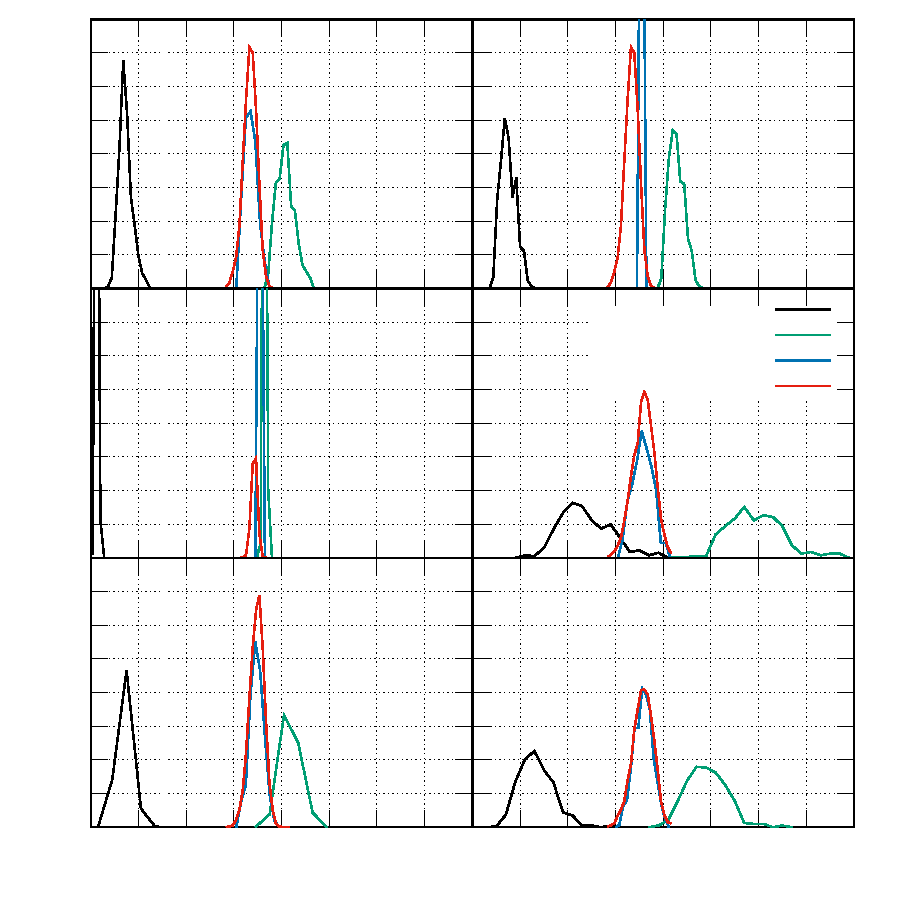
\includegraphics[width={432.00bp},height={432.00bp}]{Einitot}}%
    \gplfronttext
  \end{picture}%
\endgroup
